\chapter{Tehnologii utilizate}


\section{Raspberry Pi Zero W}

Raspberry Pi este o familie de calculatoare, de mărimea unui card de credit sau mai mici, care au revoluționat industria cu prețul accesibil de doar \$25 al primei plăci. În ultimii 5 ani, acestea au dobândit o atenție foarte mare în rândul comunității \emph{Do it yourself (DIY)} datorită spectrului larg de utilizări în proiecte digitale și IoT.

Comunitatea Raspberry a crescut mult și consistent. În momentul de față, în urma căutării "Raspberry pi projects", ne sunt returnate 47.2 milioane de pagini care conțin tutoriale despre imprimante 3D, sisteme de irigare, sisteme de luat vederi, ad-blocker pentru rețea și multe altele.

În contextul versiunii Zero W (Figura 2.1), avem disponibilă o placă de mărimea unui pachet de gume: 6.5 x 3 x 0.5 cm pe care poate fi instalat un sistem de operare bazat pe GNU/Linux numit Raspbian OS. Are un procesor single-core de 1GHz, 512 MB LPDDR2 RAM, iesire mini HDMI, două porturi micro USB, Bluetooth 4.0 și 2.4GHz 802.11n Wi-Fi.

Aspectul special al acestor computere constă în cei 40 pini \textbf{GPIO} (\emph{General purpose input-output}). Aceștia sunt folosiți pentru conectarea de senzori, fiind ușor programabili cu ajutorul limbajului Python, sau pentru audiențe tinere, Scratch.


\begin{figure}[h]
	\centering
	
\includegraphics[width=1\textwidth]{raspberrypi}
	\caption{Fața și spatele plăcii Raspberri Pi Zero W
		Credits: RPISpy @ \url{https://www.raspberrypi-spy.co.uk/}}
	\label{fig:raspberrypi}
\end{figure}

\break

\section{Microcontrollere folosite}

Un microcontroller (abreviat \emph{MCU}) este un circuit integrat care combină funcționalitate microporcesorului (de obicei aflat sub un radiator de aluminiu pentru disiparea căldurii) cu componentele periferice: module \emph{Input/output}, memorie și interfețe de comunicare cu alte module. Dețin mai mulți pini de tip analog, digital și \textbf{PWM} (\emph{Pulse Width Modulation}) pentru conectarea cu alte module

\subsection{Arduino Nano}

Arduino Nano (Figura 2.2) este fratele mai mic al plăcii Uno cu care împărtășește majoritatea funcționalității: microcontroller ATmega328, 32KB memorie flash, viteză de 16MHz și 22 pini I/O.  Singurele diferențe sunt mărimea redusă și portul de USB mini. Este perfect pentru persoanele care doersc să învețe tainele electronicii și a programării, fiind potrivit pentru proiecte ce au constrângeri legate de spațiul disponibil.

\begin{figure}[h]
	\centering
	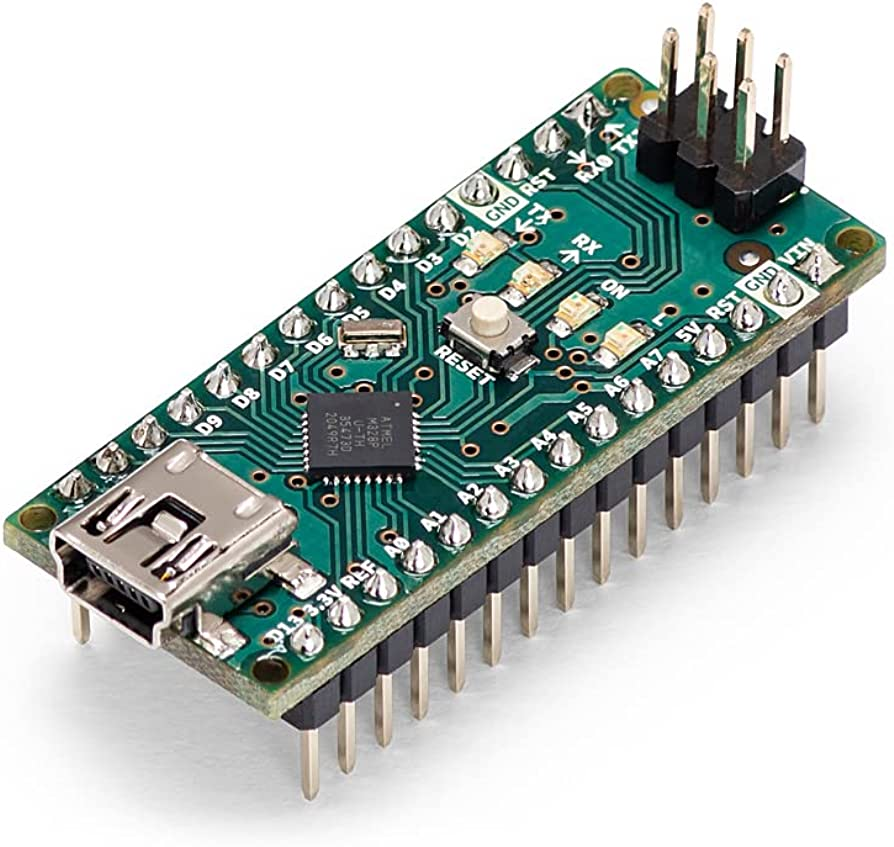
\includegraphics[width=0.4\textwidth]{arduino}
	\caption{Arduino Nano \newline\url{https://www.amazon.com/Arduino-A000005-ARDUINO-Nano/dp/B0097AU5OU}}
	\label{fig:arduino}
\end{figure}

\subsection{ESP8266}

Arduino Nano (Figura 2.2) este fratele mai mic al plăcii Uno cu care împărtășește majoritatea funcționalității. Singurele diferențe sunt mărimea redusă și portul de USB mini. Este perfect pentru persoanele care doersc să învețe tainele electronicii și a programării, fiind potrivit pentru proiecte ce au constrângeri legate de spațiul disponibil.

\begin{figure}[h]
	\centering
	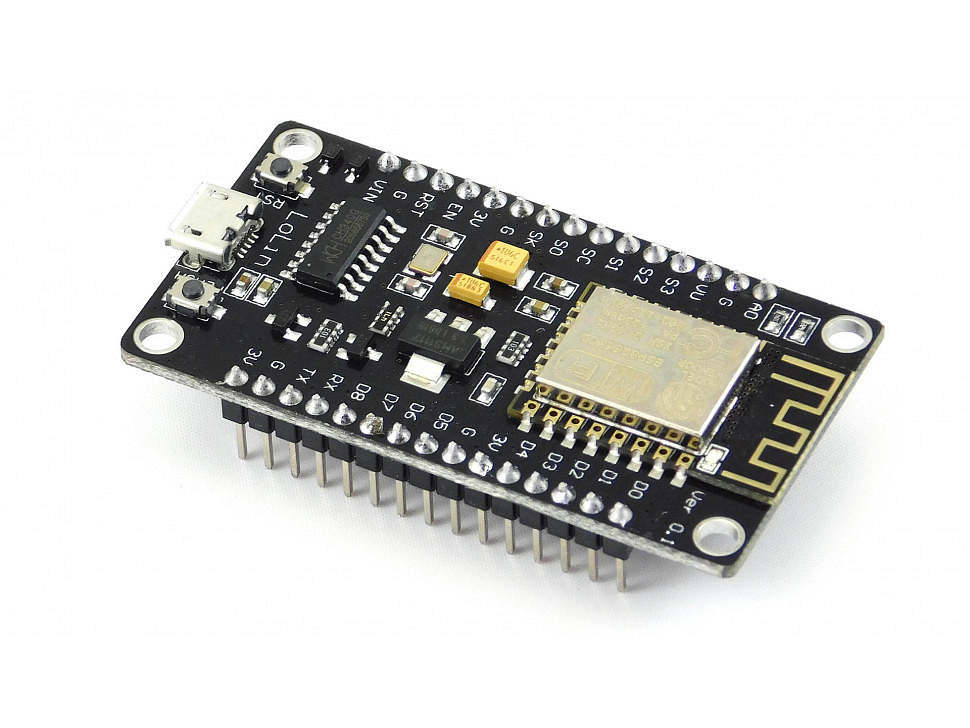
\includegraphics[width=1\textwidth]{esp8266}
	\caption{Microcontroller-ul ESP8266 (chip-ul argintiu) pe o placă de tipul \emph{Breakout} \newline\url{https://www.teachmemicro.com/esp8266-spiffs-web-server-nodemcu/}}
	\label{fig:esp8266}
\end{figure}

\break

\section{Titlul secțiunii 3}

Faucibus ornare suspendisse sed nisi lacus sed. Mi in nulla posuere sollicitudin aliquam ultrices. Lacus suspendisse faucibus interdum posuere lorem ipsum dolor sit amet. Odio tempor orci dapibus ultrices in iaculis nunc sed augue. Congue eu consequat ac felis donec et odio. Enim ut sem viverra aliquet eget sit amet. Sit amet consectetur adipiscing elit duis tristique sollicitudin. Quis blandit turpis cursus in. Cras fermentum odio eu feugiat pretium nibh ipsum consequat nisl. Non curabitur gravida arcu ac tortor dignissim convallis aenean. Porta non pulvinar neque laoreet suspendisse interdum consectetur libero id. Lacus viverra vitae congue eu consequat ac felis. Vulputate dignissim suspendisse in est ante in nibh mauris. Amet mauris commodo quis imperdiet massa. Varius sit amet mattis vulputate enim nulla aliquet. Pellentesque diam volutpat commodo sed egestas egestas. Amet est placerat in egestas erat imperdiet sed euismod. Scelerisque varius morbi enim nunc faucibus a pellentesque sit. Ut sem viverra aliquet eget sit amet tellus cras. Sem integer vitae justo eget magna fermentum iaculis eu.